\scanpage{104}
\figure{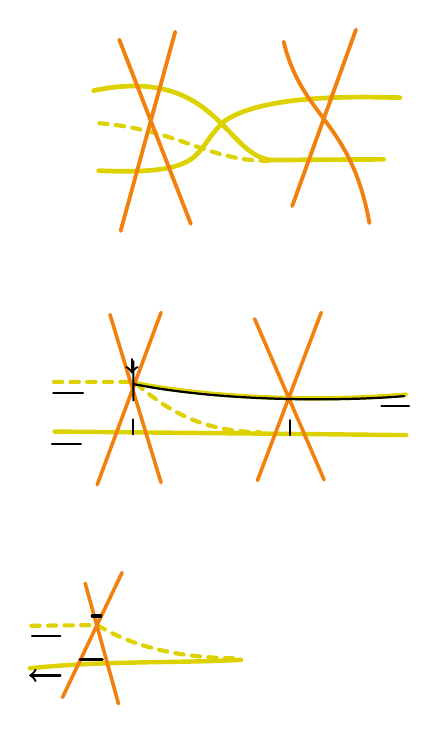
\begin{tikzpicture}[x=.009cm,y=-.009cm,line cap=round,line join=round]
\draw[yellow!70!olive,line width=1.7pt] (329,229)..controls(502,193)and(514,320)..(579,327)--(738,326) (336,342)..controls(497,349)and(466,313)..(515,271)..controls(569,236)and(688,237)..(761,239);
\draw[yellow!70!olive,line width=1.5pt,dashed] (337,275)..controls(451,285)and(492,329)..(576,328);
\draw[orange!80!brown,line width=1.4pt] (365,157)--(466,417) (444,146)--(367,427) (597,160)..controls(623,268)and(692,271)..(718,416) (699,143)--(609,392);
\draw[yellow!70!olive,line width=1.6pt] (274,710)--(770,715) (384,641)..controls(489,662)and(636,669)..(769,658);
\draw[yellow!70!olive,line width=1.5pt,dashed] (273,640)--(386,640)..controls(431,679)and(480,710)..(563,711);
\draw[orange!80!brown,line width=1.3pt] (352,545)--(424,782) (424,542)--(334,785) (556,551)--(654,778) (650,542)--(560,779);
\draw[black,line width=.8pt] (385,611)--(385,666) (385,643)..controls(515,669)and(686,667)..(767,660);
\draw[black,->,line width=.8pt] (272,656)--(314,656) (311,728)--(270,728) (385,714)--(385,693) (606,715)--(606,694) (774,674)--(735,674) (383,608)--(383,628);
\draw[yellow!70!olive,line width=1.6pt] (239,1044)..controls(342,1033)and(445,1037)..(537,1032);
\draw[yellow!70!olive,line width=1.5pt,dashed] (241,984)--(334,983)..controls(392,1018)and(462,1030)..(536,1030);
\draw[orange!80!brown,line width=1.3pt] (317,924)--(364,1094) (369,909)--(285,1085);
\draw[black,line width=1.2pt] (327,970)--(339,970) (310,1032)--(341,1032);
\draw[black,->,line width=.8pt] (242,998)--(282,998) (282,1054)--(238,1054);
\end{tikzpicture}}

Opération de rotation autour d'une face
par une flèche de transition

$(\unsure{\overleftarrow D|D},\omega,a)$, $D$ position relative\inserted{orientée}, $a$ arc de transition sur $\widetilde D$, on
trouve $(D',\omega',a')$ où
\deleted{on balaye sur l'arc de transition,}

a) $D'$ \unsure{déduite|déduit} de $D$ en \unsure{transit$^t$ suiv$^t$} $a$

b) $\omega'$ est l'orientat. \uline{opposée} à celle déduite de $\omega$ par transport

c) $a'$ est l'arc de transition sur $\widetilde D'$, qui \uline{suit} l'arc de
transition transporté de $a$, dans la direction $\omega'$.

\uline{NB} Le balayage du \unsure{lieu} de spécialisation

Le balayage de l'arc de spécialisation

l'antibalay. par des
\figure{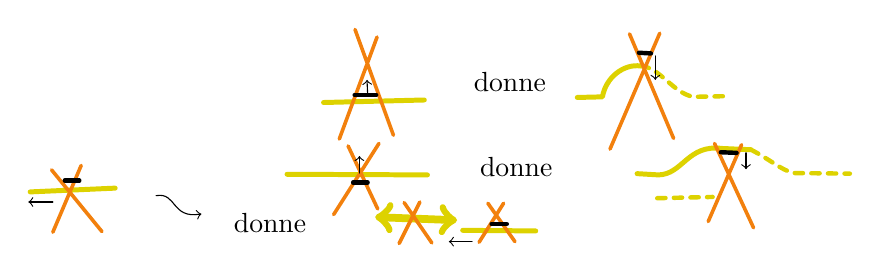
\begin{tikzpicture}[x=.008cm,y=-.008cm,line cap=round,line join=round]
\draw[yellow!70!olive,line width=1.8pt] (1989,928)--(2149,924);
\draw[orange!80!brown,line width=1.3pt] (2039,812)--(2100,980) (2074,824)--(2014,986);
\draw[black,line width=1.4pt] (2038,916)--(2073,916);\draw[black,->] (2059,914)--(2058,892);
\node at (2285,895) {donne};
\draw[yellow!70!olive,line width=1.8pt] (2392,920)--(2432,919)..controls(2437,889)and(2465,866)..(2493,870);
\draw[yellow!70!olive,line width=1.6pt,dashed] (2493,870)..controls(2523,872)and(2543,912)..(2576,919)--(2624,918);
\draw[orange!80!brown,line width=1.3pt] (2475,819)--(2545,985) (2523,818)--(2444,1002);
\draw[black,line width=1.6pt] (2490,849)--(2509,850);\draw[black,->] (2516,854)--(2516,892);
\draw[yellow!70!olive,line width=1.8pt] (1931,1042)--(2154,1043);
\draw[orange!80!brown,line width=1.3pt] (2028,997)--(2075,1097) (2077,993)--(2005,1106);
\draw[black,line width=1.6pt] (2036,1055)--(2059,1055);\draw[black,->] (2046,1040)--(2046,1013);
\node at (2295,1030) {donne};
\draw[yellow!70!olive,line width=1.8pt] (2487,1041)--(2521,1043)..controls(2560,1042)and(2567,994)..(2622,1001)--(2668,1003);
\draw[yellow!70!olive,line width=1.6pt,dashed] (2668,1003)..controls(2699,1019)and(2714,1034)..(2735,1040)--(2825,1041) (2519,1080)--(2607,1078);
\draw[orange!80!brown,line width=1.3pt] (2610,993)--(2672,1127) (2653,995)--(2600,1117);
\draw[black,line width=1.6pt] (2620,1007)--(2645,1008);\draw[black,->] (2660,1008)--(2660,1034);
\draw[yellow!70!olive,line width=1.8pt] (1523,1070)--(1658,1064);
\draw[orange!80!brown,line width=1.3pt] (1557,1035)--(1637,1133) (1604,1028)--(1559,1134);
\draw[black,line width=1.6pt] (1578,1052)--(1601,1052);\draw[black,->] (1559,1086)--(1520,1086);
\draw[black,->] (1723,1076)..controls(1756,1070)and(1747,1113)..(1795,1105);
\node at (1904,1120) {donne};
\draw[yellow!70!olive,line width=2.8pt,<->] (2071,1110)--(2201,1115);
\draw[orange!80!brown,line width=1.3pt] (2117,1087)--(2161,1151) (2142,1086)--(2109,1152);
\draw[yellow!70!olive,line width=1.8pt] (2210,1131)--(2326,1132);
\draw[orange!80!brown,line width=1.3pt] (2250,1088)--(2293,1149) (2275,1088)--(2236,1150);
\draw[black,line width=1.6pt] (2256,1121)--(2280,1121);\draw[black,->] (2225,1149)--(2188,1149);
\end{tikzpicture}}

Pour $\rho(D,\omega,-)=(D',\omega',a')$, \deleted{\unsure{les}}\inserted{\unsure{quatre}} cas à considérer se groupent par deux paires,
correspondant resp. aux cas où $a$ est un arc de spécialisation, un arc de généralisation
\figure{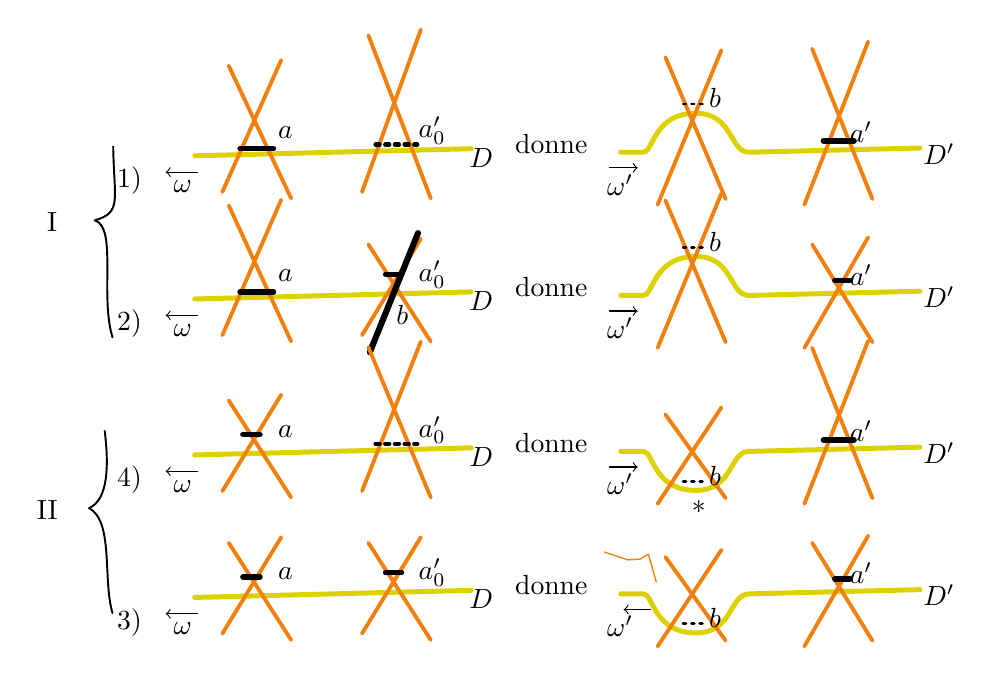
\begin{tikzpicture}[x=.009cm,y=-.009cm,line cap=round,line join=round]
\draw[yellow!70!olive,line width=1.8pt] (650,1458)--(1040,1448);
\draw[orange!80!brown,line width=1.4pt] (698,1331)--(786,1518) (772,1323)--(689,1509);
\draw[orange!80!brown,line width=1.4pt] (895,1288)--(983,1518) (969,1280)--(886,1509);
\draw[black,line width=2pt] (714,1448)--(761,1448);
\node at (778,1425) {$a$};\node at (985,1423) {$a_0^{\prime}$};\node at (1054,1461) {$D$};\node at (558,1493) {1)};\node at (1153,1441) {donne};
\draw[black,->] (654,1481)--(609,1481);\node at (633,1502) {$\omega$};
\draw[black,dotted,line width=1.5pt] (905,1442)--(964,1442);
\draw[yellow!70!olive,line width=1.8pt] (1251,1453)--(1283,1453)..controls(1297,1453)and(1297,1398)..(1357,1398)..controls(1410,1398)and(1404,1453)..(1432,1453)--(1673,1447);
\draw[orange!80!brown,line width=1.4pt] (1314,1319)--(1399,1519) (1393,1309)--(1303,1527);
\draw[orange!80!brown,line width=1.4pt] (1521,1307)--(1606,1519) (1600,1297)--(1510,1527);
\node at (1384,1377) {$b$};\node at (1590,1424) {$a^{\prime}$};\node at (1700,1455) {$D^{\prime}$};
\draw[black,line width=2pt] (1537,1437)--(1580,1437);
\draw[black,dotted,line width=1pt] (1339,1385)--(1373,1385);
\draw[black,->] (1235,1475)--(1275,1475);
\node at (1250,1499) {$\omega^{\prime}$};
\draw[yellow!70!olive,line width=1.8pt] (650,1660)--(1040,1650);
\draw[orange!80!brown,line width=1.4pt] (698,1528)--(786,1720) (772,1520)--(689,1711);
\draw[orange!80!brown,line width=1.4pt] (895,1583)--(983,1720) (969,1575)--(886,1711);
\draw[black,line width=2pt] (714,1650)--(761,1650);
\node at (778,1627) {$a$};\node at (985,1625) {$a_0^{\prime}$};\node at (1054,1663) {$D$};\node at (558,1695) {2)};\node at (1153,1643) {donne};
\draw[black,->] (654,1683)--(609,1683);\node at (633,1704) {$\omega$};
\draw[black,line width=1.8pt] (919,1625)--(942,1625);
\draw[black,line width=2.2pt] (897,1735)--(965,1567);\node at (943,1683) {$\unsure{b}$};
\draw[yellow!70!olive,line width=1.8pt] (1251,1655)--(1283,1655)..controls(1297,1655)and(1297,1600)..(1357,1600)..controls(1410,1600)and(1404,1655)..(1432,1655)--(1673,1649);
\draw[orange!80!brown,line width=1.4pt] (1314,1521)--(1399,1721) (1393,1511)--(1303,1729);
\draw[orange!80!brown,line width=1.4pt] (1521,1583)--(1606,1721) (1600,1573)--(1510,1729);
\node at (1384,1579) {$b$};\node at (1590,1626) {$a^{\prime}$};\node at (1700,1657) {$D^{\prime}$};
\draw[black,line width=2pt] (1553,1634)--(1574,1634);
\draw[black,dotted,line width=1pt] (1339,1587)--(1373,1587);
\draw[black,->] (1235,1677)--(1275,1677);
\node at (1250,1701) {$\omega^{\prime}$};
\draw[yellow!70!olive,line width=1.8pt] (650,1880)--(1040,1870);
\draw[orange!80!brown,line width=1.4pt] (698,1803)--(786,1940) (772,1795)--(689,1931);
\draw[orange!80!brown,line width=1.4pt] (895,1728)--(983,1940) (969,1720)--(886,1931);
\draw[black,line width=2pt] (718,1851)--(742,1851);
\node at (778,1847) {$a$};\node at (985,1845) {$a_0^{\prime}$};\node at (1054,1883) {$D$};\node at (558,1915) {4)};\node at (1153,1863) {donne};
\draw[black,->] (654,1903)--(609,1903);\node at (633,1924) {$\omega$};
\draw[black,dotted,line width=1.5pt] (905,1864)--(964,1864);
\draw[yellow!70!olive,line width=1.8pt] (1251,1875)--(1283,1875)..controls(1297,1875)and(1297,1930)..(1357,1930)..controls(1410,1930)and(1404,1875)..(1432,1875)--(1673,1869);
\draw[orange!80!brown,line width=1.4pt] (1314,1823)--(1399,1941) (1393,1813)--(1303,1949);
\draw[orange!80!brown,line width=1.4pt] (1521,1729)--(1606,1941) (1600,1719)--(1510,1949);
\node at (1384,1909) {$b$};\node at (1590,1846) {$a^{\prime}$};\node at (1700,1877) {$D^{\prime}$};
\draw[black,line width=2pt] (1537,1859)--(1580,1859);
\draw[black,dotted,line width=1pt] (1339,1917)--(1373,1917);
\draw[black,->] (1235,1897)--(1275,1897);
\node at (1250,1921) {$\omega^{\prime}$};
\node at (1361,1954) {$\unsure{*}$};
\draw[yellow!70!olive,line width=1.8pt] (650,2081)--(1040,2071);
\draw[orange!80!brown,line width=1.4pt] (698,2004)--(786,2141) (772,1996)--(689,2132);
\draw[orange!80!brown,line width=1.4pt] (895,2004)--(983,2141) (969,1996)--(886,2132);
\draw[black,line width=2pt] (718,2052)--(742,2052);
\node at (778,2048) {$a$};\node at (985,2046) {$a_0^{\prime}$};\node at (1054,2084) {$D$};\node at (558,2116) {3)};\node at (1153,2064) {donne};
\draw[black,->] (654,2104)--(609,2104);\node at (633,2125) {$\omega$};
\draw[black,line width=1.8pt] (919,2046)--(942,2046);
\draw[yellow!70!olive,line width=1.8pt] (1251,2076)--(1283,2076)..controls(1297,2076)and(1297,2131)..(1357,2131)..controls(1410,2131)and(1404,2076)..(1432,2076)--(1673,2070);
\draw[orange!80!brown,line width=1.4pt] (1314,2024)--(1399,2142) (1393,2014)--(1303,2150);
\draw[orange!80!brown,line width=1.4pt] (1521,2004)--(1606,2142) (1600,1994)--(1510,2150);
\node at (1384,2110) {$b$};\node at (1590,2047) {$a^{\prime}$};\node at (1700,2078) {$D^{\prime}$};
\draw[black,line width=2pt] (1553,2055)--(1574,2055);
\draw[black,dotted,line width=1pt] (1339,2118)--(1373,2118);
\draw[black,->] (1293,2098)--(1255,2098);
\node at (1250,2122) {$\omega^{\prime}$};
\draw[black,line width=.7pt] (535,1445)..controls(536,1520)and(548,1538)..(509,1549)..controls(541,1559)and(516,1655)..(534,1714);
\draw[black,line width=.7pt] (523,1846)..controls(529,1895)and(528,1943)..(501,1955)..controls(536,1974)and(520,2056)..(534,2103);
\node at (449,1551) {$\mathrm{I}$};\node at (442,1958) {$\mathrm{II}$};
\draw[orange!80!brown,line width=.5pt] (1228,2017)--(1261,2028)--(1278,2027)--(1290,2020)--(1301,2059);
\end{tikzpicture}}
Dans tous les cas, pour déterminer
$a'$, on peut soit prendre l'arc $a'_0$\inserted{de transition}
qui suit $a$ sur $\widetilde D$ dans la direction
\uline{opposée} à $\omega$, et prendre son \uline{transporté}
par balayage\inserted{ou antibalayage}; soit transporter d'abord
$a$ en $b$ par la dite opération, et prendre
le successeur de $b$ pour $\omega'$, parmi
les arcs de transition sur $\widetilde D'$.
Cela résulte du fait que dans une
opération de spécialisation, l'isom can. entre
$\mathrm{Pol}(D)$ et $\mathrm{Pol}(D')$ induit une bijection entre
l'ens. des arcs de transition sur le premier,
\margin{103}
